\chapter{Preliminaries}\label{chapter:preliminaries}

\emph{Space weather} is the branch of physics that studies the time varying phenomena in the solar 
system. The principal driver of space weather phenomena is the Sun, specifically its magnetic field 
variations and the \emph{solar wind}. The effect of solar variations on the planetary environment 
are caused by the coupling between solar wind particles and the magnetic field produced by the 
Earth. This chapter gives a semi-quantitative treatment of various scientific ideas relevant to 
space weather research.

\begin{table}
    \centering
    \begin{tabular}{l p{0.35\textwidth} r}
        \hline
        \textbf{Chapters} & \textbf{Themes} & \textbf{Recommended Reading}\\
        \hline
        \vspace{5pt}
        \ref{chapter:dst_osa} \& \ref{chapter:dst_msa} & Forecasting of geomagnetic index $\mathrm{Dst}$. & \S~\ref{sec:geoindex}, \S~\ref{sec:mag}\textsuperscript{*}, \S~\ref{sec:plasma}\textsuperscript{*} \\
        \ref{chapter:bayes_diff_chapter} & Inference of radiation belt parameters. & \S~\ref{sec:plasmadiff}, \S~\ref{sec:plasma}\textsuperscript{*} \S~\ref{sec:mag}\textsuperscript{*} \\
        \ref{chapter:pdt} & Forecasting of near Earth solar wind speed using solar data. & \S~\ref{sec:hmfsolarwind}, \S~\ref{sec:sunspots}, \S~\ref{sec:solar}\textsuperscript{*}\\
        \hline
    \end{tabular}
    \caption{Dissertation Guide. {\small Asterisk\textsuperscript{*} denotes optional material.}}
    \label{table:chapterguide}
\end{table}

\Cref{table:chapterguide} provides the reader with a condensed guide to this dissertation. 
It connects the content presented in this chapter with the main research problems analyzed in the 
later chapters and provides recommended prerequisite reading for each chapter.

Section \S~\ref{sec:plasma} describes space plasmas and their properties. Section 
\S~\ref{sec:solar} provides some background about the Sun and the solar wind which is the driver 
for all space weather phenomena. This is used in the solar wind prediction task considered in 
\cref{chapter:pdt}. Section \S~\ref{sec:plasmadiff} introduces the plasma diffusion model 
(\cref{eq:fokker}) and its simplified radial diffusion system (\cref{eq:radialDiff}) which is 
used as the underlying physical model for \cref{chapter:bayes_diff_chapter}. Section 
\S~\ref{sec:mag} introduces the \emph{magnetosphere}, giving context for 
\cref{chapter:dst_osa,chapter:dst_msa}. 


\section{Space Plasma}\label{sec:plasma}

Plasma, also known as the fourth state of matter due to its properties that differentiate it 
from the conventional gaseous state, is ubiquitous throughout the visible Universe. Plasma is a gas 
which is composed of roughly equal number of positive and negatively charged particles, a property 
known as charge \emph{quasi-neutrality}. The term quasi-neutral is used because although the gas 
has almost equal amounts of positive and negative charges, the mixture is electromagnetically 
active. Due to incomplete charge shielding, long range electromagnetic fields play a big role in 
the dynamics of plasma.

%From classical electrostatics the electric potential of a point charge $q$, is given as

%\begin{equation}
%    \phi(r) = \frac{q}{4\pi\epsilon_0 ||r||_2}
%\end{equation}

%where $r$ is the position in space with respect to the charge and $\epsilon_0$ is the \emph{permittivity} of vacuum.

\subsection*{Debye Length}

In a quasi-neutral plasma, due to the presence of partial electric shielding the potential due to 
the charges now takes the well known Debye form
%
\begin{equation}
    \phi(r) = \frac{q}{4\pi\epsilon_0 r} e^{-\frac{r}{\lambda_d}} \ , 
\end{equation} 
%
where $r$ is the spatial distance with respect to the charge and $\epsilon_0$ is the 
\emph{permittivity} of vacuum. The electric potential decays with the Debye length scale 
$\lambda_d$ at which a balance between thermal vibrations which can disturb quasi-neutrality, and 
electrostatic forces due to charge separation, is achieved. The Debye length scale depends on the 
electron temperature and plasma density.
%
\begin{equation}\label{eq:debye}
    \lambda_d = \sqrt{\frac{\epsilon_0 k_b T_e}{n_e e^2}}
\end{equation}
%
In \cref{eq:debye} above, the Debye length scale is expressed in terms of the 
\emph{Boltzmann constant} $k_b$, the electron temperature $T_e$, free space permittivity 
$\epsilon_0$, and electron charge $e$. One can visualise the positively charged ions having a cloud 
of electrons shielding them at the distance of $\lambda_d$. 

It is also possible to take into account the shielding effect of the ions. The effective Debye 
length is now expressed as an addition of two terms: one for electrons (\cref{eq:debye}) and a 
similar term for the ions by replacing $T_e$ for the ion temperature $T_i$ ($n_i \approx n_e$). 

\subsection*{Plasma Parameter}

Consider a Debye sphere of radius $\lambda_d$. This sphere contains 
$N_e = \frac{4}{3}\pi \lambda^3_d n_e$ electrons. The plasma parameter $g$ is defined as 
$N_{e}^{-1}$. Rewriting this, we can say:
%
\[
    g \sim \sqrt{\frac{n_e}{T_e}} \ .
\]
%
The description of plasma used in many applications in space is applicable when $g \ll 1$. In 
this situation the Debye shielding is significant, and the quasi-neutral plasma obeys collective 
statistical behavior. The plasma parameter $g$ also correlates with the collision frequency. The 
collisions in plasma increase with increasing density and decreasing temperature, and if 
$g \longrightarrow 0$ the plasma becomes nearly collisionless. The collisionless property helps in 
making simplifying assumptions about plasma dynamics and serves as the starting point for the 
\emph{adiabatic} theory of plasma motions in the Earth's magnetosphere which will be discussed in 
section \S~\ref{sec:plasmadiff}.

\section{Sun \& the Solar Wind}\label{sec:solar}

\begin{figure}
    \noindent\centering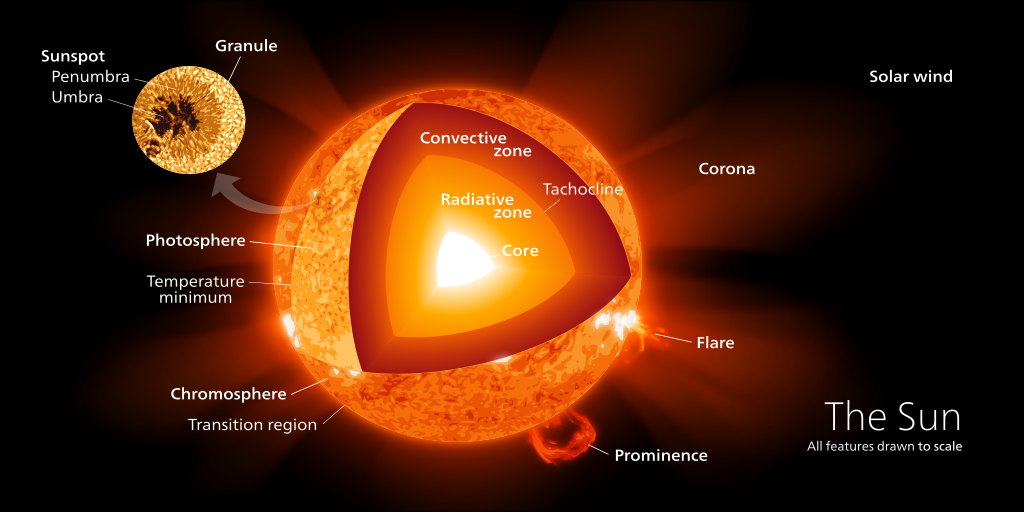
\includegraphics[width=\textwidth]{Sun_poster.png}
    \caption{{\small Cross section of the Sun \\ 
    Author: Kelvinsong [CC BY-SA 3.0 (\url{https://creativecommons.org/licenses/by-sa/3.0})]}}
    \label{fig:SunLayers}
\end{figure}

The Sun is an almost perfectly spherical ball of plasma which is the the center of our solar 
system and the only source of light and energy for all living and meteorological processes on 
Earth. Apart from terrestrial weather, the Sun is also the primary driver of space weather which 
results from the interaction between the solar wind and planetary magnetospheres.

\subsection{Structure}

\Cref{fig:SunLayers} shows a cross section of the Sun with various layers. We give a brief 
description of them below.

\textbf{Core}: The core of the Sun is the site for the thermonuclear fusion reactions which produce 
its energy. It extends from the center to about $20-25\%$ of the solar radius \citep{SolarAct}. It 
has a temperature close to $\SI{1.57d7}{\kelvin}$ and a density of 
$\SI{150}{\gram\per\centi\metre^3}$ \citep{SolarCore}. Nuclear fusion in the core takes place via 
the well known \emph{proton-proton chain} (pp).

\textbf{Radiative Zone}: The radiative zone extends from $25\%$ to $70\%$ of the solar radius. 
The nuclear reactions in the core are highly sensitive to temperature and pressure. In fact, they 
are almost shut off at the edge of the core. In the radiative zone, energy transfer takes place via 
photons (radiation) which bounce around nuclei until they reach the convective zone.

\textbf{Convective Zone}: The convective zone lies between $70\%$ of the solar radius to a point 
close to the solar surface. Density decreases dramatically going from the core to the radiative 
zone and subsequently the convective zone. In this region, the solar material behaves more like a 
fluid. Due to the temperature gradient which exists across it, the primary source of transport is 
here via convection.

\textbf{Photosphere}: The photosphere is the visible \enquote{surface} of the Sun, since the layers 
below it are all opaque to visible light. A layer of about $\SI{100}{\kilo\metre}$ thickness, the 
photosphere is also the region from where sunlight can freely escape into space. The photospheric 
surface has a number of features i.e. sunspots, granules and faculae. Sunspots (see section 
\S~\ref{sec:sunspots}) are magnetic regions where the solar material has a lower temperature 
compared to its surroundings. Magnetic field lines are concentrated in sunspot regions, and the 
field strength in sunspots can often be thousands of times stronger than the on the Earth.

% \begin{wrapfigure}{r}{0.4\textwidth}
%     \centering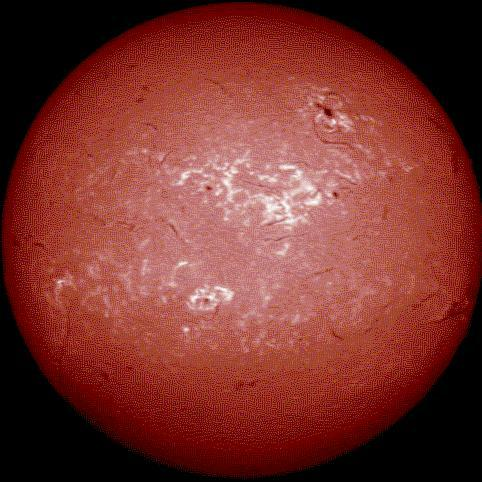
\includegraphics[width=0.38\textwidth]{chromosphere.jpg}
%     \caption{
%         {\small Chromosphere viewed using an $H\alpha$ filter. \\ \textit{Source}: CWitte (Public domain)}}
%     \label{fig:chromosphere}
% \end{wrapfigure}

\begin{wrapfigure}{r}{0.4\textwidth}
    \centering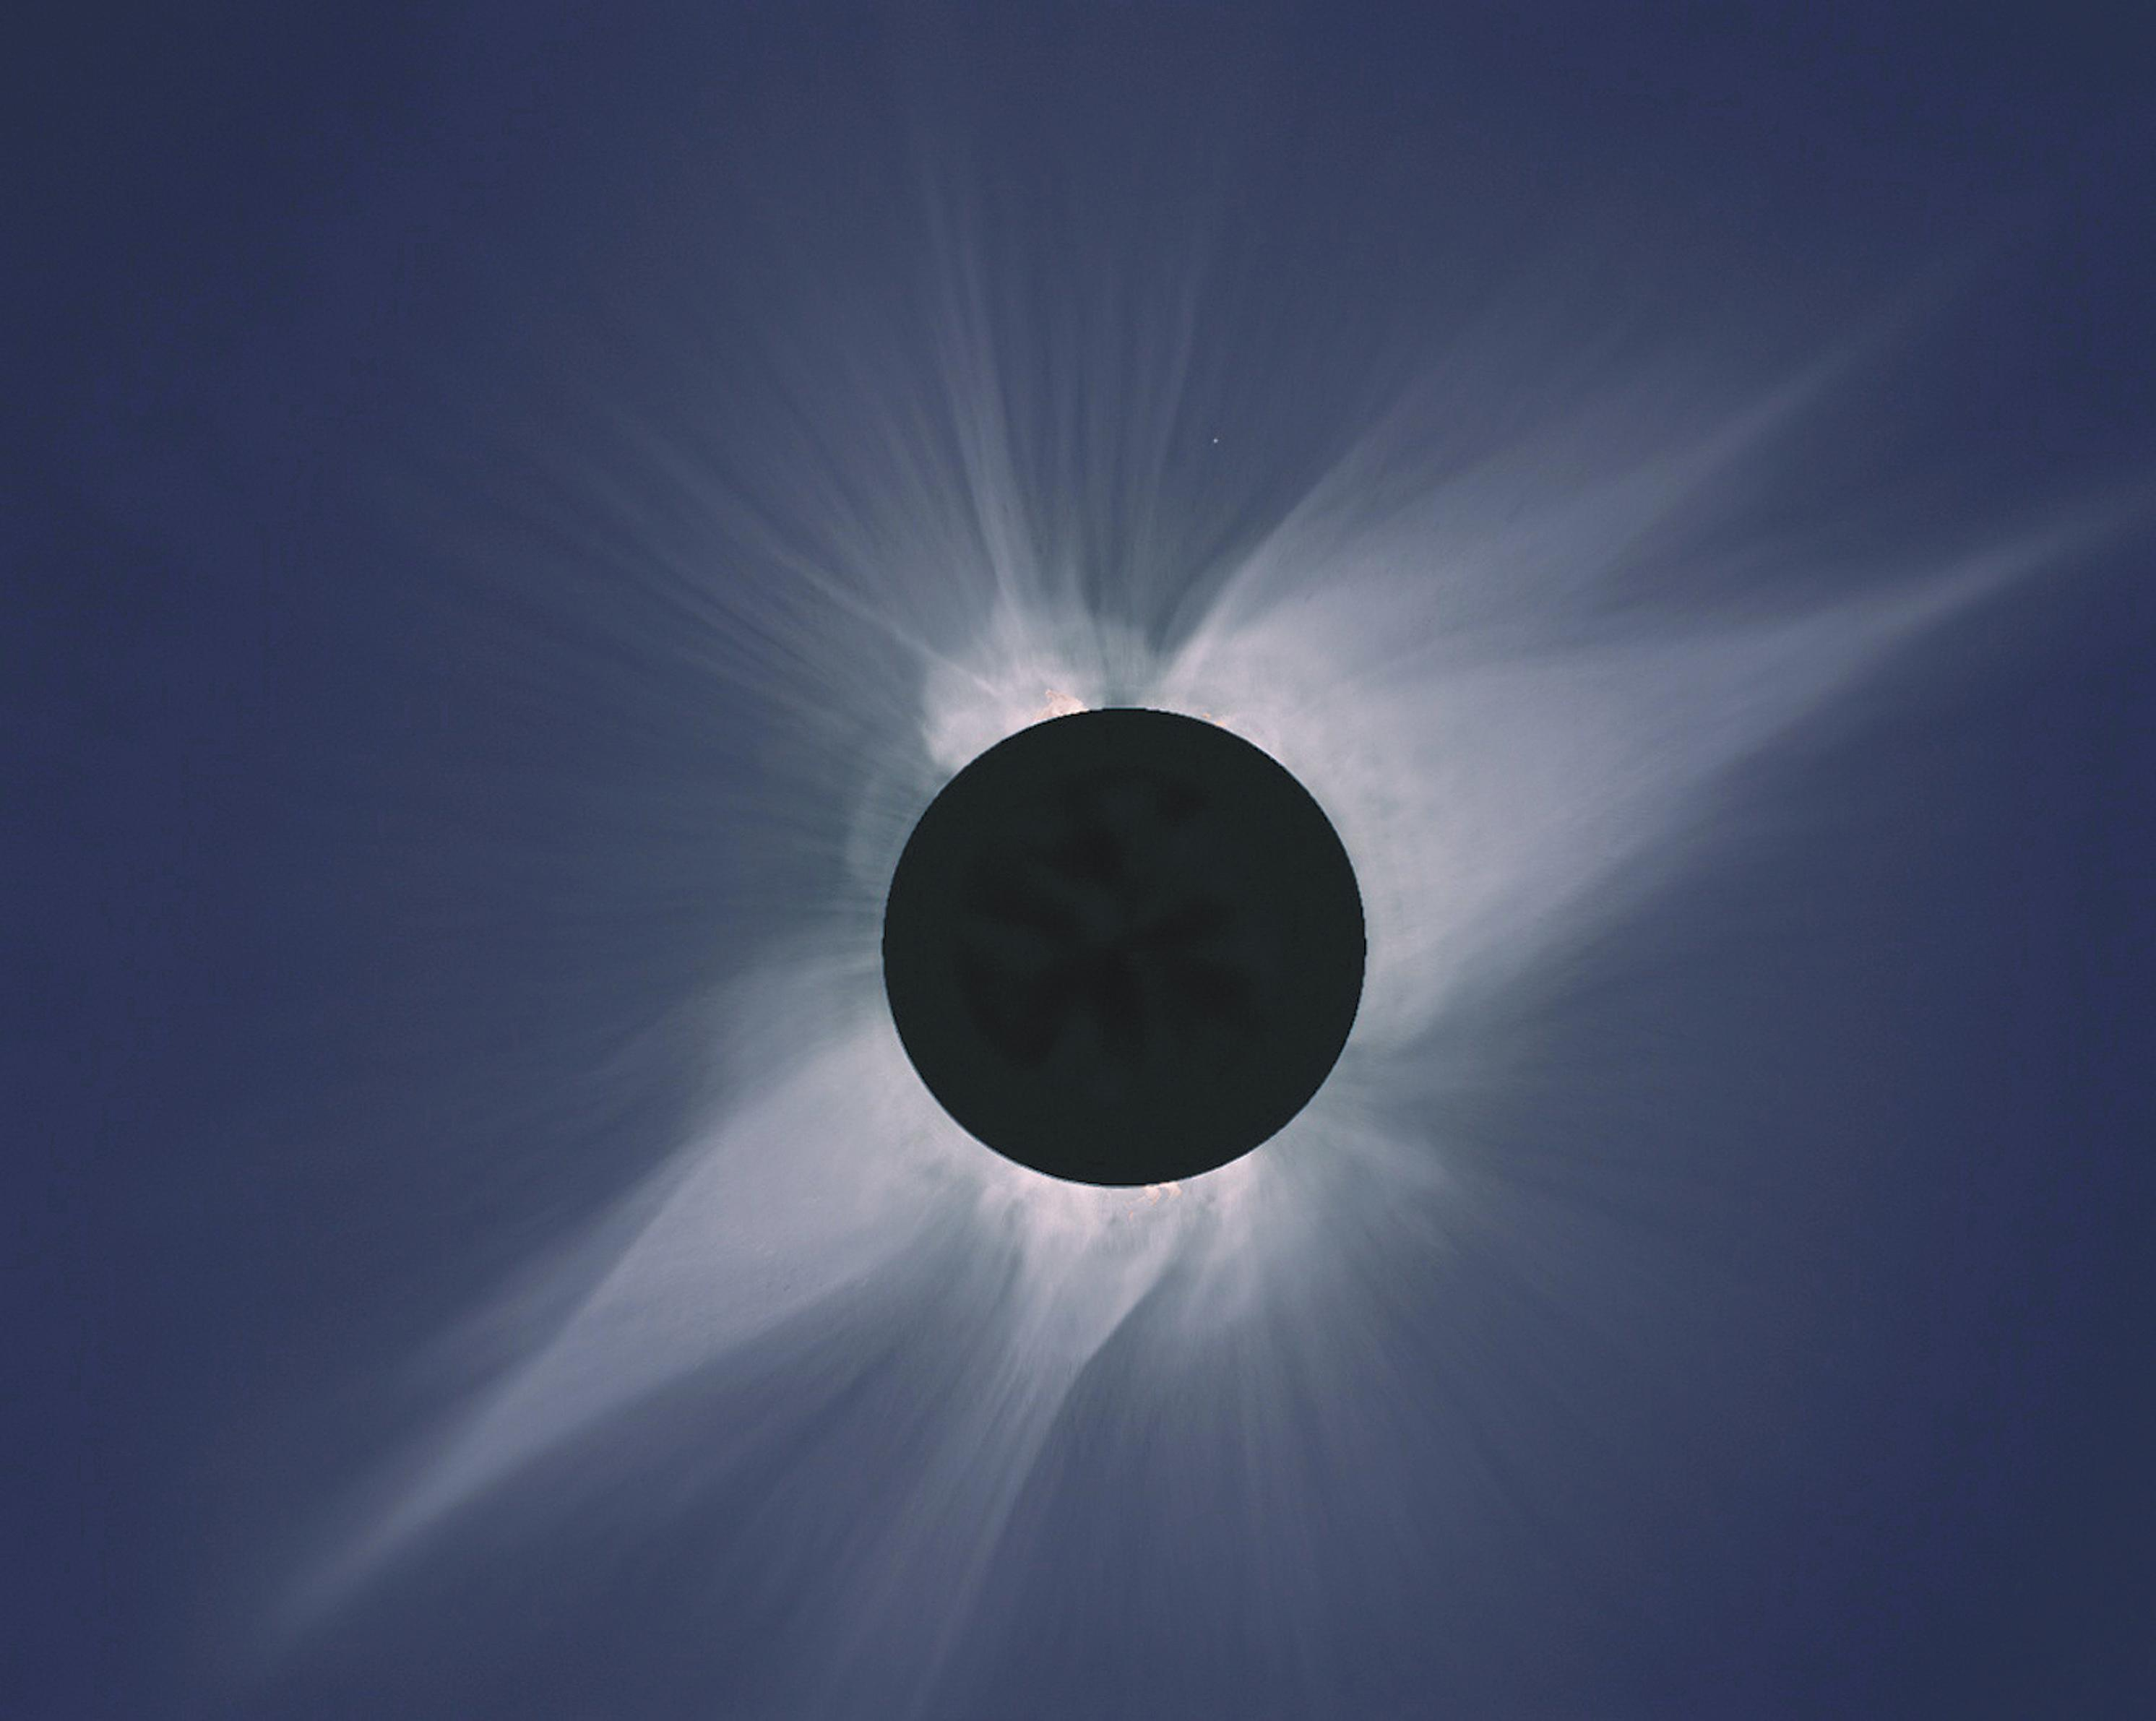
\includegraphics[width=0.38\textwidth]{coronaBaja.jpg}
    \caption{
        {\small 
            Sun's corona captured during a solar eclipse. \\ 
            \textit{Source}: Steve Albers, Boulder, CO; Dennis DiCicco, Sky and Telescope; 
            Gary Emerson, E. E. Barnard Observatory
        }
    }
    \label{fig:coronaBaja}
\end{wrapfigure}


\textbf{Chromosphere}: The Chromosphere extends for a distance of almost $\SI{5000}{\kilo\metre}$ 
after the photosphere. The chromosphere is known for the existence of features called spicules and 
prominences. The chromosphere has a red colour which is generally not visible due to the intense 
light given off by the photosphere but can be observed through a filter centered on the Hydrogen 
$H\alpha$ spectral line. %(see figure \ref{fig:chromosphere}). 

\textbf{Solar Transition Region}: A thin ($\SI{100}{\kilo\metre}$) region between the chromosphere 
and the solar corona where the temperature rises from about \SIrange{8000}{5d5}{\kelvin}, the solar 
transition region might not be well defined at all altitudes; however its existence is evidenced by 
a bifurcation of the dynamics of the solar plasma. Below the transition region, the dynamics is 
dictated by gas pressure, fluid dynamics, and gravitation while above the region, the dynamics is 
dictated more by magnetic forces.

\textbf{Corona}: An aura of plasma around the Sun that extends millions of kilometers into space, 
the corona can be observed during a total solar eclipse (\cref{fig:coronaBaja}) or with a 
coronagraph. The temperature of the corona is dramatically higher than the photosphere and 
chromosphere. The average temperature can range from \SIrange{1d6}{2d6}{\kelvin} while in the 
hottest regions it can be as high as $\SI{2d7}{\kelvin}$ \citep{SolarCorona}. Although the reason 
for this dramatic increase is still not well understood, there exist various explanations using 
concepts of magnetic reconnection \citep{russell2001solar,SolarCorona} and Alfv\'en waves 
\citep{AlfvenCorona}. There is a critical height in the corona, known as the \emph{source surface}, 
below which the magnetic field controls the plasma completely. Above it the plasma carries 
the magnetic field with it into the interplanetary medium.


\subsection{Solar Wind \& Heliospheric Magnetic Field}\label{sec:hmfsolarwind}

The idea that the Sun was ejecting charged particles outwards into space was first hinted at after 
the solar storm of $1859$ by Richard Carrington \citep{cliver20131859} and later by George 
FitzGerald \citep{meyer2007basics}. Arthur Eddington, in a footnote of an article about the comet 
Morehouse in $1910$, was the first to suggest the existence of the solar wind, without naming it so 
\citep{eddingtonFootnote}.

In the $1950\text{s}$, studies of the anti-solar orientation of the ion tails of Halley's comet 
led to the theory of solar corpuscular emission \citep{Bierman1,Bierman2,Bierman3}. 
\citet{parker1958dynamics,Parker1960,Parker1965} argued that the corona cannot remain in 
hydrostatic equilibrium and that supersonic expansion of the corona is responsible for the 
outward expulsion of charged particles, which the author referred to as the \emph{solar wind}.

\citet{parker1958dynamics} also proposed a spiral model for the \emph{Heliospheric Magnetic Field} 
(HMF) and suggested that the solar wind carried with it the solar magnetic field. The Parker model 
was further supported its ability to explain the effect of the HMF on the modulation of galactic 
cosmic rays and their measured intensities close to the Earth \citep{ParkerSolarWind}. In $1959$ 
the Soviet spacecraft Luna $1$ was the first to directly observe the solar wind and measure its 
strength \citep{harvey2007russian}. Subsequently, the Mariner $2$ mission recorded properties of 
the positive ion component of the solar wind and confirmed the Parker spiral HMF model 
\citep{neugebauer1966mariner}.

The structure of the HMF is central to explaining the formation and propagation of the solar wind. 
The HMF in steady state points radially outward and rotates with the Sun, producing an 
\emph{Archimedean spiral} structure as postulated in \cite{parker1958dynamics} and shown 
schematically in \cref{fig:parkerspiral}. Photospheric observations of the magnetic field (see 
Global Oscillation Network Group \url{https://gong.nso.edu}) are often extrapolated to compute 
approximations to the coronal HMF topology. There exist a number of techniques used to perform such 
extrapolations: potential field based methods such as \emph{Potential-Field Source Surface} (PFSS) 
\citep{schatten1969model,altschuler1969magnetic}, PFSS variants such as 
\emph{Potential-Field Current Sheet} (PFCS) \citep{schatten1971current}, 
\emph{Current-Sheet Source Surface} (CSSS) \citep{csss}, and several others. Apart from potential 
based models, there exist more involved techniques based on Magnetohydrodynamics (MHD) such as 
\emph{Magnetohydrodynamics Around a Sphere} (MAS) \citep{linker1999magnetohydrodynamic}, 
ENLIL \citep{ODSTRCIL1996,ODSTRCIL1999a,ODSTRCIL1999b,ODSTRCIL2003,ODSTRCIL2004} and EUHFORIA 
\citep{pomoell2018euhforia}. 

The HMF can be seen as a combination of two components: the poloidal magnetic field and the 
toroidal magnetic field. The two fields often exchange energy between themselves over the course of 
several years in a cyclical phenomenon known as the \emph{solar cycle} (section 
\S~\ref{sec:sunspots}). Interested readers can read \citet{Owens2013} for an in-depth review on the 
phenomena that drive the HMF. \todo{\textbf{TODO}: Check that the HMF image can be reproduced here.}

\begin{figure}
    \noindent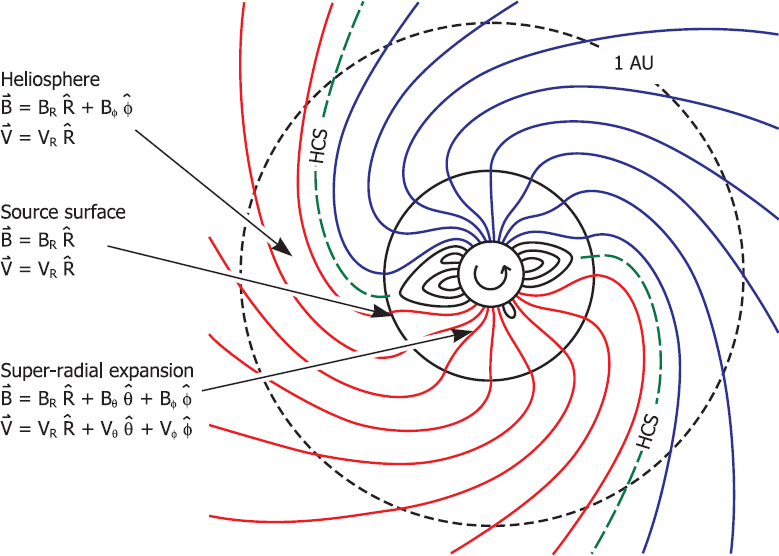
\includegraphics[width=0.8\textwidth]{parker-spiral.jpg}
    \caption{
        {\small 
            An illustration of the Heliospheric Magnetic Field in the \emph{ecliptic plane}. In the 
            heliosphere, rotation of the HMF foot points within a radial solar wind flow generates 
            an azimuthal component of the HMF, $B_{\phi}$, leading to a spiral geometry. Red and 
            blue lines, showing regions of opposite polarity, are separated by the heliospheric 
            current sheet (HCS), shown as the green dashed line. Image reproduced from 
            \citet{Owens2013}
        }
    }\label{fig:parkerspiral}
\end{figure}


The expansion of the coronal magnetic field leads to an eventual opening of field lines at the 
source surface (see \cref{fig:parkerspiral}) and the ejection of the solar wind. This hot plasma 
consists mostly of protons, electrons and a small number of helium and heavy ions. The solar wind 
spirals outwards in all directions, carrying with it the magnetic field. Close to the Earth's 
magnetosphere, this wind has a nominal speed of about $\SI{400}{\kilo\metre\per\second}$ while its 
high speed component has an average velocity of $\sim \SI{700}{\kilo\metre\per\second}$ 
(\cref{fig:solarwinddist}).

\begin{figure}
    \noindent\centering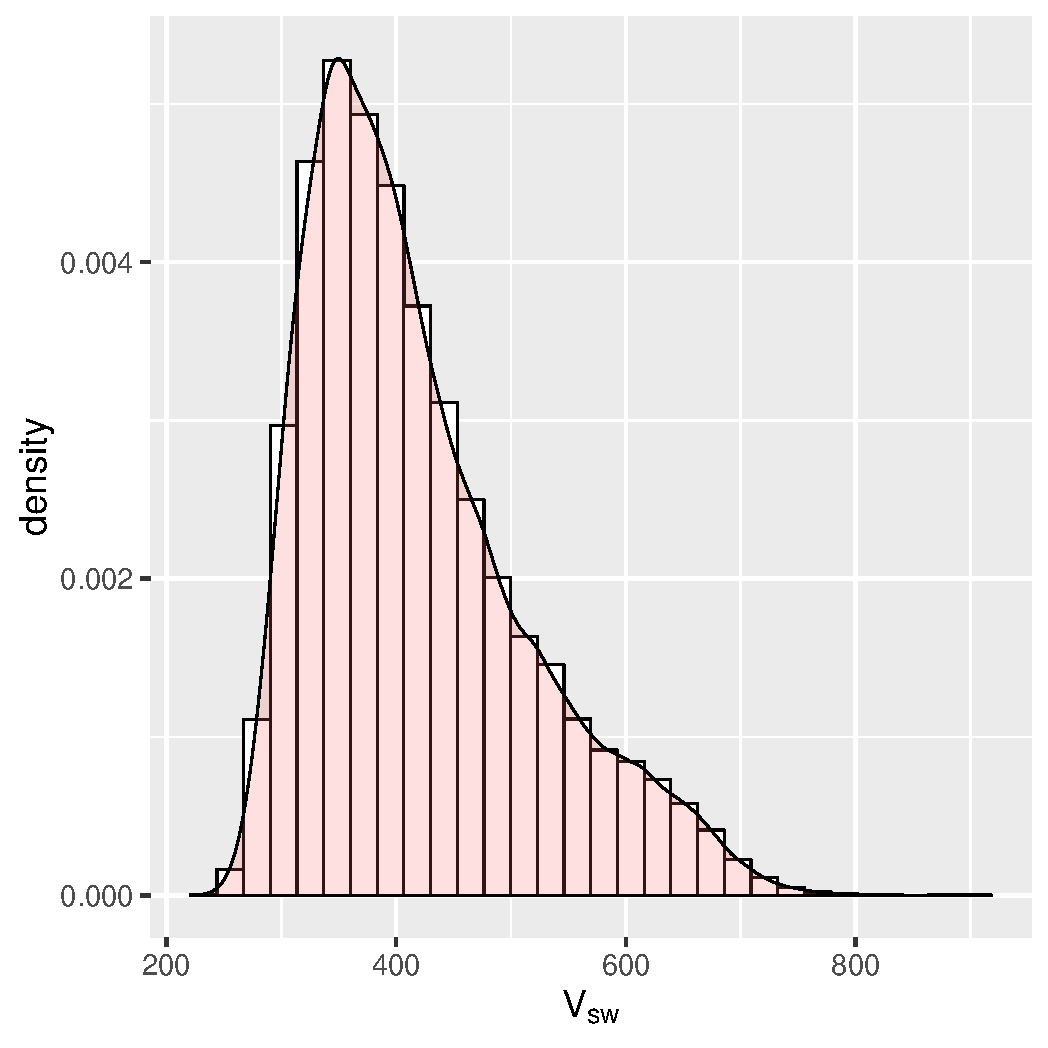
\includegraphics[width=0.75\textwidth]{solarwinddist.pdf}
    \caption{
        {\small 
            Distribution of solar wind speed recorded at $\SI{1}{\astronomicalunit}$ for the time 
            period $2008 - 2018$, \textit{Source}: OMNI data set 
            (\url{https://omniweb.gsfc.nasa.gov/ow.html})
        }
    }\label{fig:solarwinddist}
\end{figure}

\subsubsection*{Near Earth Measurements}

The solar wind has the heliospheric magnetic field \emph{frozen in} \footnote{the flux of the 
magnetic field going through a surface that moves with the solar wind (in a Lagrangian manner) is 
constant}, and as it propagates in the interplanetary medium, it carries the solar magnetic field 
with it \citep{alfven1942existence,alfven1943existence}. Important solar wind quantities such as: 
%
\begin{enumerate*} 
    \item solar wind speed, 
    \item proton density, and  
    \item magnetic field strength 
\end{enumerate*}
% 
are recorded at the well known $L1$ \emph{Lagrangian point} where the gravitational fields of the 
Earth and the Sun approximately balance out.



\subsection{Sunspots \& Solar Cycle}\label{sec:sunspots}

Sunspots are temporarily occurring regions on the Sun's photosphere that appear as dark spots. 
They are areas of magnetic field concentration where the field lines often \enquote{puncture} the 
solar surface inhibiting convection and producing regions with lower temperatures than the 
surroundings. Sunspots generally last anywhere between a few days to a few months. They can occur 
in pairs or groups and can accompany other phenomena such as \emph{coronal loops}, 
\emph{prominences}, and reconnection events.

Since the $19^{\text{th}}$ century the number of sunspots on the Sun's surface have been recorded 
as the \emph{sunspot number} (SSN). Sunspots populations increase and decrease, thereby behaving as 
markers for solar activity levels. The cyclical behavior of sunspot populations is called the 
\emph{sunspot cycle} or \emph{solar cycle} (\cref{fig:SolarCycle}). 

\begin{figure}
    \noindent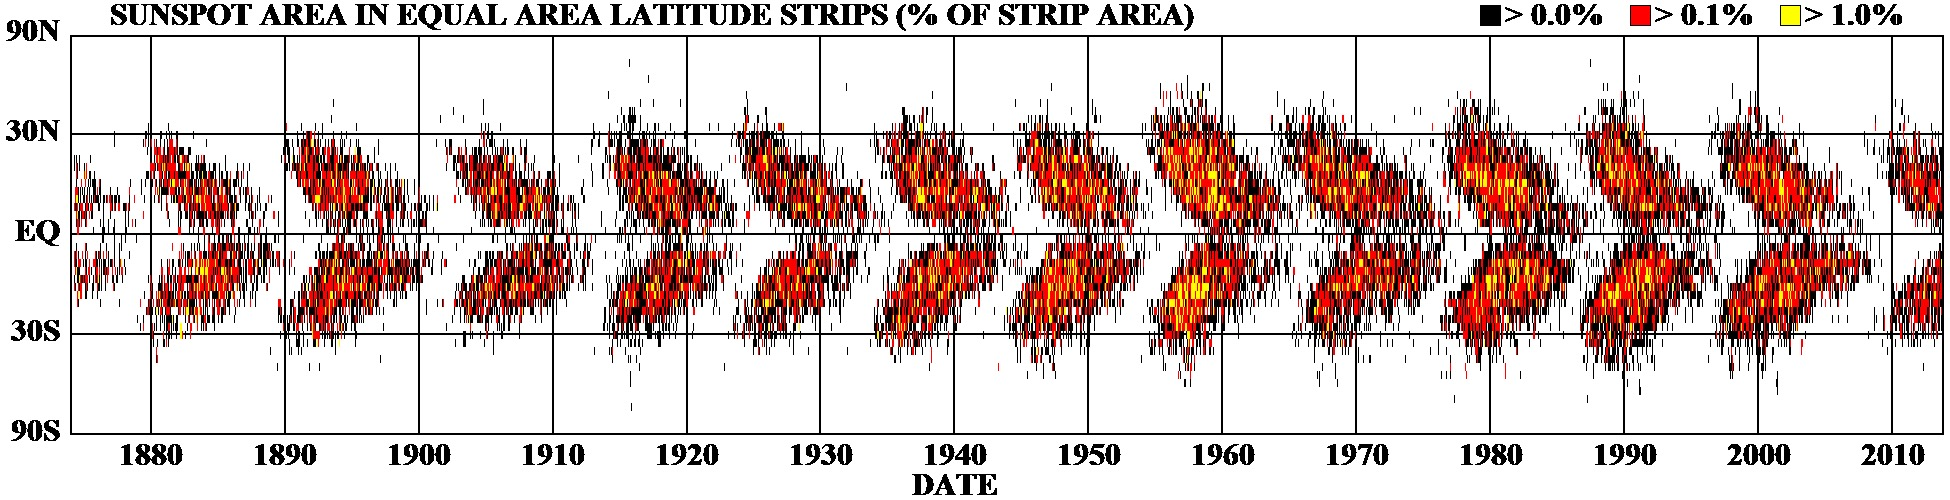
\includegraphics[width=\textwidth]{sunspot-cycle.jpeg}
    \caption{{\small The sunspot butterfly diagram.  \\ 
    \textit{Author}: David Hathaway, NASA, Marshall Space Flight Center (Public domain) \\ 
    \textit{Source}: Wikipedia}}
    \label{fig:SolarCycle}
\end{figure}

\Cref{fig:SolarCycle} depicts how the area occupied by sunspots changes with solar latitude 
and time. During the start of a solar cycle (solar minimum), sunspots start appearing at higher 
latitudes. Over the course of the cycle, they move towards the equatorial regions and their number 
increases to some maximum (solar maximum). Towards the end, the number of sunspots diminishes and 
the entire cycle starts over. This repetitive behavior happens over approximately $11$ years.

Because sunspots are magnetic phenomena, the solar cycle represents cyclical behavior of the HMF. 
During solar minimum, the poloidal component of the solar magnetic field is at its strongest and it 
is the closest it can get to a magnetic dipole configuration. Towards solar maximum, energy is 
transferred from the poloidal component to the toroidal component, resulting in complex field 
configurations which are evidenced by larger numbers of sunspot clusters.

The solar cycle also gives rise to variations in solar irradiance \citep{solarirradiance}. Between 
$1645$ and $1715$, a period known as the \emph{Maunder minimum}, very few sunspots were observed. 
This coincided with lower than average temperatures in Europe, which was called the 
\emph{little ice age}. Sunspot numbers going back $11000$ years have been reconstructed using 
Carbon-$14$ based analysis of tree rings. Apart from the \emph{Maunder minimum}, other periods of 
very low sunspot activity have been matched with corresponding \emph{little ice ages}.

In \cref{chapter:pdt}, the \emph{sunspot number} data as well as the \emph{flux tube expansion} 
factor ($f_S$ or FTE) and the magnetic field strength computed by the CSSS model will be used to 
create a input data set for building the \emph{dynamic time lag regression} model proposed therein. 
Using the input parameters, the \XX \ model provides an estimate for the near Earth solar wind speed 
as well as the propagation time. Measurements of the solar wind speed will also be used in 
\cref{chapter:dst_osa,chapter:dst_msa} as inputs to the Dst forecasting models applied therein.


\section{Magnetosphere}\label{sec:mag}

% \begin{figure}
%     \noindent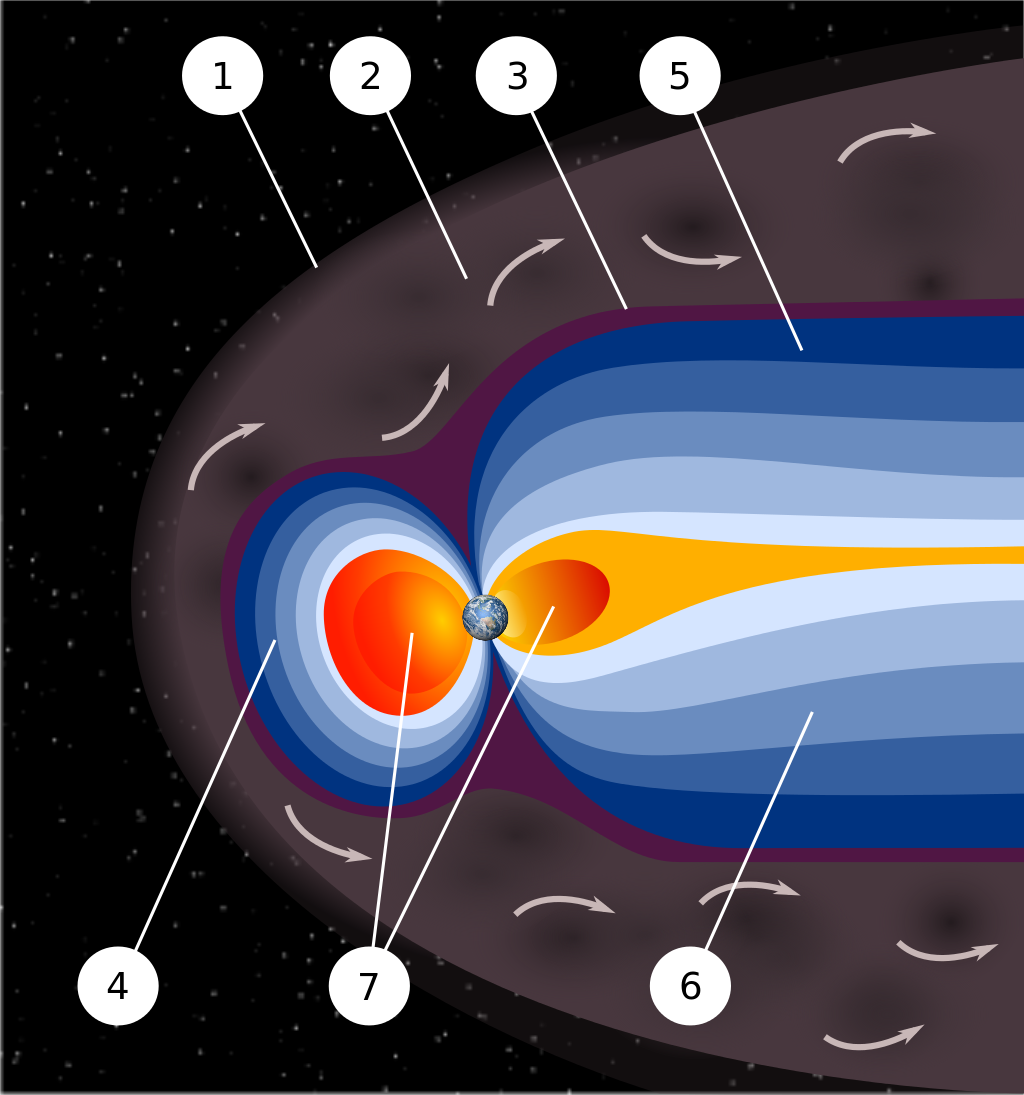
\includegraphics[width=0.7\textwidth]{mag.png}
%     \caption{{\small Schematic diagram of the Earth's magnetosphere: \\
%     The Sun (not shown) is to the left of the figure, the solar wind propagates from left to right.\\
%     1) Bow shock. 2) Magnetosheath. 3) Magnetopause. 4) Magnetosphere. \\
%     5) Northern tail lobe. 6) Southern tail lobe. 7) Plasmasphere.\\ 
%     Source: Dennis Gallagher, derivative work: Fr\'ed\'eric Michel (Public domain)}
%     }
%     \label{fig:magnetosphere}
% \end{figure}

\begin{figure}[ht]
    \noindent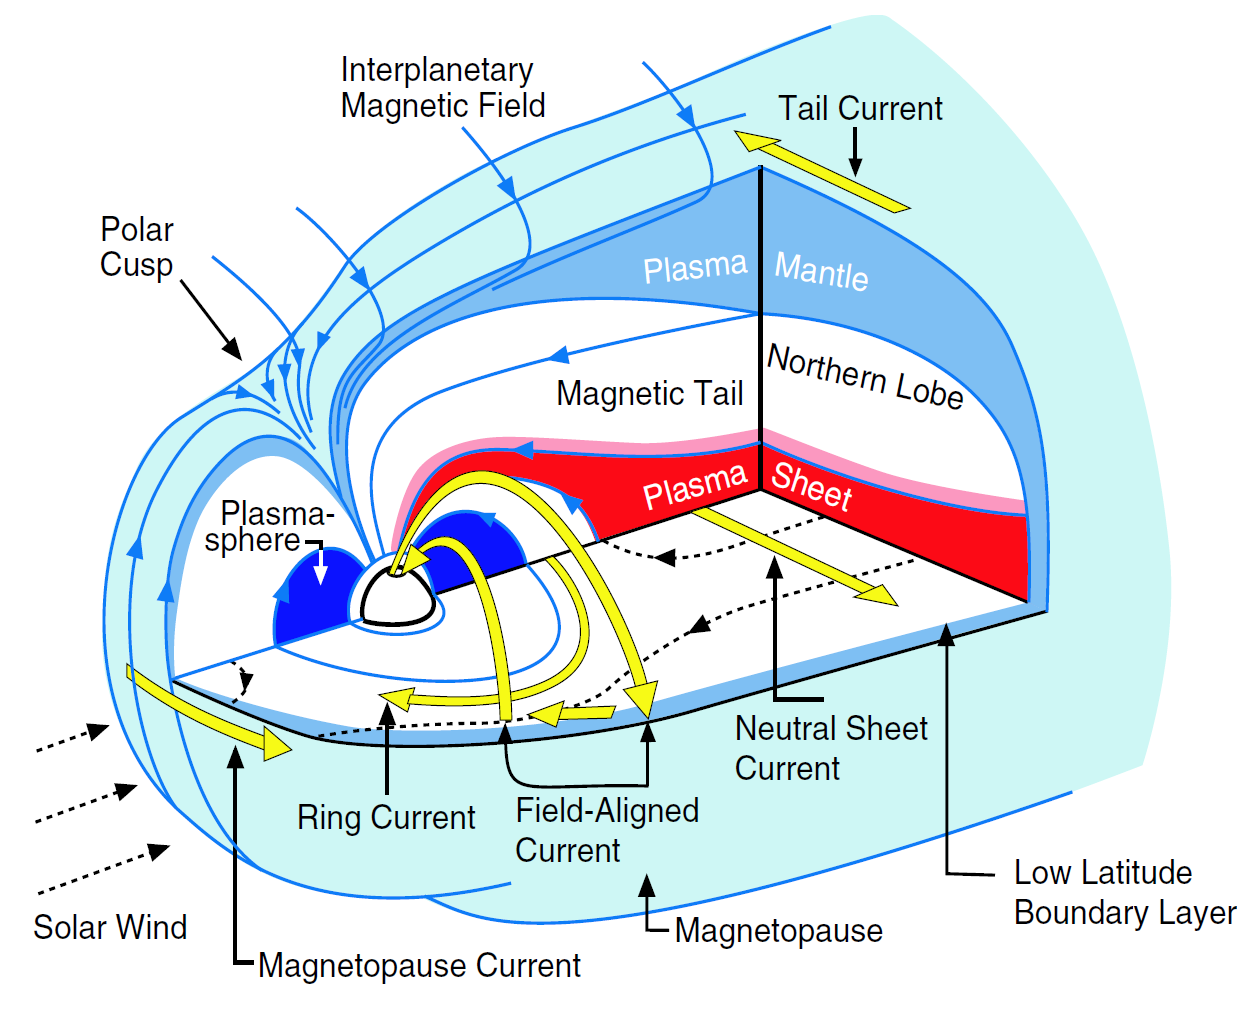
\includegraphics[width=0.8\textwidth]{mag3.png}
    \caption{
        {\small 
            Three-dimensional cutaway view of the magnetosphere. The light blue outer surface is 
            the magnetopause, and its boundary layers are shown in darker blue. Magnetic field lines 
            are shown in blue, electric currents in yellow. The polar region where the magnetic 
            field lines converge is the polar cusp. The bow shock has been omitted for clarity. 
            Reproduced from \citet{DeKeyser2005}
        }
    }
    \label{fig:magnetosphere}
\end{figure}

The Earth's magnetosphere (\cref{fig:magnetosphere}) is a region surrounding the planet where its 
magnetic field dominates the \emph{interplanetary magnetic field}. The Earth's magnetic field 
shields the atmosphere and terrestrial life from the impact of the solar wind. 

As the solar wind approaches the Earth, it is slowed down and deflected by the Earth's magnetic 
field. Since the solar wind is supersonic when it arrives and slows down to subsonic levels, a 
shock wave is generated in the process (\emph{bow shock}). Much of the solar wind kinetic energy is 
converted to thermal energy when it crosses the \emph{bow shock} into the \emph{magnetosheath}. The 
\emph{magnetosheath} spans from the \emph{bow shock} to the \emph{magnetopause}. The 
\emph{magnetopause} is the outer boundary of the Earth's magnetic shield. Its location is 
$\sim 10R_E$ ($R_E = \SI{6372}{\kilo\metre}$, the radius of the Earth). 


Earth's magnetic shielding is not perfect, and some particles manage to get trapped inside the 
cavity of the \emph{magnetosphere}. This region of trapped plasma is known as the the 
\emph{van Allen radiation belts}. Particles trapped in the radiation belts execute complex motions 
which can be approximately modelled using ideas from adiabatic theory and diffusion described in 
section \S~\ref{sec:plasmadiff} below. The \emph{plasmasphere} is the inner region of the radiation 
belts which contains cold, dense plasma. The portion of the magnetosphere facing away from the Sun 
(called the \emph{nightside}) is stretched out in a tail-like shape by the deflected solar wind, 
hence referred to as the \emph{magnetotail}. The \emph{magnetotail} has an approximate extent 
of up to $1000R_E$.


\subsection{Particle Motions \& Adiabatic Theory} \label{sec:plasmadiff}

This section gives a quick introduction to the theory of charged particle motions in the 
magnetosphere. The reader may refer to \citet{roederer2012dynamics} for an in depth treatment of 
this subject. To understand the motions of charged particles in the \emph{magnetosphere}, the role 
of electric and magnetic forces must be understood.

It is well known from classical electromagnetism that the force exerted on a particle with charge 
$q$ by a magnetic field $\mathbf{B}$ and an electric field $\mathbf{E}$ is given by the well known 
\emph{Lorentz force} (\cref{eq:lorentzforce}).
%
\begin{equation}\label{eq:lorentzforce}
    \mathbf{F} = m\frac{d\mathbf{v}}{dt} = q\mathbf{E} + q\mathbf{v} \times \mathbf{B}
\end{equation}
%
The first component of \cref{eq:lorentzforce} ($q\mathbf{E}$) is either parallel or opposite to the 
local electric field depending on the charge of the particle. The second component 
$q\mathbf{v} \times \mathbf{B}$ involves a vector cross product so it is always perpendicular to 
the plane spanned by vectors $\mathbf{v}$ and $\mathbf{B}$. In order to understand its effects, we 
can decompose the particle velocity in two components; $v_{\parallel}$ parallel to $\mathbf{B}$ and 
$v_{\perp}$ perpendicular to $\mathbf{B}$. If $\mathbf{E} = \mathbf{0}$, then the particle executes 
a circular motion with properties shown in \cref{eq:larmor}. Here $\rho$ is the gyroradius and 
$\omega$ is the gyrofrequency or cyclotron frequency. In the case where $v_{\parallel} \neq 0$, the 
trajectory is helical.
%
\begin{equation}\label{eq:larmor}
    \frac{v^{2}_{\perp}}{\rho} = \frac{qBv_{\perp}}{m} = \omega v_{\perp}
\end{equation}
%
Apart from the gyro motion, there are some important drift forces that significantly influence 
particle motions.
%
\begin{itemize}
    \item Electric field drift: If $\mathbf{E}$ has a component $E_{\perp}$ perpendicular to 
    $\mathbf{B}$, the electric field accelerates and decelerates the particle in the two 
    hemispheres of the orbit. The orbit becomes a distorted circle, and the particle drifts in a 
    direction perpendicular to the electric field with a velocity 
    $\mathbf{v_d} = \mathbf{E} \times \mathbf{B} / B^2$.

    \item Magnetic gradient drift: When the magnetic field varies in space (as is the case of the 
    Earth), a gradient in the field strength in the direction perpendicular to $\mathbf{B}$ gives 
    rise to a gradient drift velocity given by 
    $\mathbf{v_g} = \frac{1}{2} m v^2_{\perp}\mathbf{B} \times \frac{\nabla \mathbf{B}}{aB^3}$.

    \item Magnetic curvature drift: If the magnetic field has a curvature, this creates an 
    additional drift motion with velocity 
    $\mathbf{v_c} = \frac{ m v_{\parallel} \mathbf{B} \times (\hat{\mathbf{b}} \cdot \nabla) 
    \hat{\mathbf{b}} }{qB^2}, \ \ \mathbf{b} = \frac{\mathbf{B}}{B}$.
\end{itemize}

The equations of motion for charged particles in the general case of spatially varying electric and 
magnetic fields do not admit closed-form solutions. The motions are generally complex and require 
lengthy numerical integrations to be resolved.
%
\begin{figure}[ht]
    \centering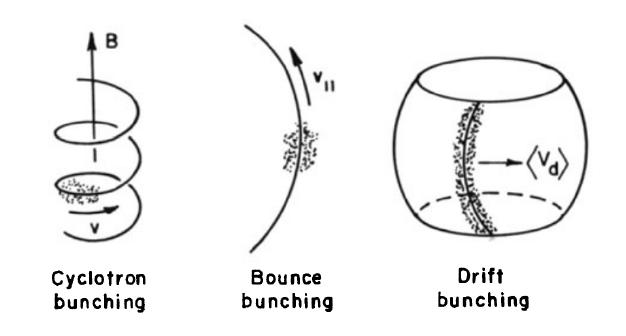
\includegraphics[width=0.4\textwidth]{adiabatic_motions.jpeg}
    \caption{
        {\small 
        Periodic components of particle motion. Reproduced from \citet{roederer2012dynamics}
        }
    }
    \label{fig:particlemotions}
\end{figure}
%
\todo{\textbf{TODO}: Check that the adiabatic motion image from Roederer can be reproduced here.}

The \emph{guiding center} approximation helps us to decompose particle motions into three periodic 
components (\cref{fig:particlemotions}):
%
\begin{enumerate*}
    \item gyration around magnetic field lines, 
    \item bounce motions between magnetic north and south poles, and
    \item equatorial drift of electrons and protons, 
\end{enumerate*}
%
each with its own time scale.

\subsubsection*{Adiabatic Invariants}

When a physical system with periodic motion is varied slowly as compared to the time period of 
its periodicity, the transformation can be characterized as \emph{adiabatic}. 
Formally speaking, for systems which are described by Hamiltonian dynamics, we can write the 
equations of motion in terms of the \emph{canonical position} $q$, the \emph{canonical momentum} 
$p$, external parameters $\theta$, and the system's \emph{Hamiltonian} $\mathcal{H}(q,p|\theta)$: 
%
\begin{equation}\label{eq:hamilton}
    \begin{aligned}
        \dot q &= \frac{\partial \mathcal{H}}{\partial p}\\
        \dot p &= - \frac{\partial \mathcal{H}}{\partial q} \ .
    \end{aligned}
\end{equation}
%
If the system shown in \cref{eq:hamilton} executes a periodic motion in the $q,p$ phase 
space, it admits an \emph{adiabatic invariant} $A$ given in \cref{eq:adiabatic_invariant}.
%
\begin{equation}\label{eq:adiabatic_invariant}
    A = \oint p d q
\end{equation}
%
The quantity $A$ would remain approximately constant if the external parameters $\theta$ were 
varied adiabatically (i.e. if changes in $\theta$ happen over a time period much greater than 
the period of oscillation of the system).

Applying the idea of adiabatic invariance to charged particle motion in the \emph{magnetosphere}, 
it is possible to associate one adiabatic invariant with each periodic motion i.e. gyromotion 
$\mathcal{M}$, bounce $J$, and drift $\Phi$ (\cref{eq:plasmainv}). 
%
\begin{align}\label{eq:plasmainv}
    \mathcal{M} &= \frac{1}{2}\frac{mv^{2}_{\perp}}{\rvert \mathbf{B} \rvert} \\
    J &= \oint{m_0 v_{\parallel}ds} \\
    \Phi &= \oint{v_{\text{drift}} \cdot r d\phi} = \int{\mathbf{B} d\mathbf{S}}
\end{align}
%
The first invariant $\mathcal{M}$ is associated with the Larmor gyration - it is the magnetic 
moment of the current generated by the circular motion of the particle around the field line. 

The second invariant $J$ is associated with the bounce motion between the two magnetic mirrors near 
the north and south poles (the quantity $s$ is an appropriately chosen arc length coordinate along 
the bounce trajectory). The bounce motion between the magnetic poles can be explained by the 
conservation of the particle energy $\frac{1}{2}m v^2_{\parallel} + \frac{1}{2}m v^{2}_{\perp}$ and 
the first invariant $\mathcal{M}$. Because field strength $\rvert \mathbf{B} \rvert$ increases 
near the poles, $v_{\perp}$ also increases to conserve $\mathcal{M}$; however, to conserve energy, 
$v_{\parallel}$ decreases until the particle can no longer move farther along the field line (and 
bounces back).

The third invariant $\Phi$, associated with equatorial drift motion, is actually the magnetic 
flux through the barrel shape envelope of the particle drift. A particle's guiding magnetic field 
line can be identified by its radial position $r$ and its longitude $\phi$. The magnetic flux of 
the drift can then be computed by integrating over $\phi$.

Associated with each adiabatic invariant is a timescale which determines how easily its 
conservation can be violated. The timescales for $\mathcal{M},\ J, \ \text{and} \ \Phi$ are the 
time periods of the gyromotion, bounce motion, and equatorial drift motion respectively. Since 
it takes much a longer time for the particles to complete a drift motion around the Earth as 
compared to bounce and gyromotion (in that order), the invariance of $\Phi$ is most easily 
violated - a fact which is used in the simplification of the Fokker-Planck diffusion system 
described below.    

\subsubsection*{Plasma Diffusion}

Because we consider populations of charged particles, it is natural to employ some kind of 
distribution based picture for magnetospheric plasma. The adiabatic invariants give us a phase 
space or coordinate system by which we can express quantities of interest. 

The main quantity of interest in this case is the \emph{phase space density} 
$f(t, \mathcal{M}, J, \Phi)$ which is a function of time and three invariants. The 
\emph{phase space density} tells us the number of particles in a particular region of the phase 
space, and at a particular point of time.

Diffusion behavior arises when one or more of the invariants are violated, which can happen due to 
a number of reasons such as: 
%
\begin{enumerate*}
    \item non-adiabatic variations of the magnetic field, 
    \item external forces, 
    \item interaction with electromagnetic waves, and 
    \item collisions with atmosphere/ionosphere. 
\end{enumerate*}
%
The plasma diffusion system \citep{schulz2012particle} can be written as a generalized 
Fokker-Planck system as shown in \cref{eq:fokker}.
%
\begin{align}\label{eq:fokker}
    \frac{\partial{f}}{\partial{t}} &= \sum^{3}_{p,q = 1}
    \frac{\partial}{\partial{J_{p}}} \left( \kappa_{pq}
    \frac{\partial{f}}{\partial{J_{q}}} \right) \\
    J_1 &= \mathcal{M} \\
    J_2 &= J \\
    J_{3} &= \Phi
\end{align}
%
It is possible to simplify this system by considering the two main categories of diffusion: radial 
diffusion and pitch angle diffusion. Radial diffusion allows particles to move farther or closer 
to the Earth, and pitch angle \footnote{pitch angle being the angle between particle velocity 
$\mathbf{v}$ and the magnetic field $\mathbf{B}$} diffusion moves the magnetic mirror points along 
the field lines.

Rewriting $\Phi \propto \frac{1}{\ell}$, the third invariant can be expressed in terms of the 
\emph{drift shell} $l$ (larger value of $l$ implies greater distance from the Earth). The radial 
diffusion system can be obtained from \cref{eq:fokker} by keeping $\mathcal{M}\ \text{and} \ J$ 
fixed, considering diffusion in $\ell$ (violation of $\Phi$ invariance), and by approximating pitch 
angle diffusion as a loss process \citep{roederer2012dynamics,Walt1970}.  
%
\begin{equation}\label{eq:radialDiff}
    \frac{\partial{f}}{\partial{t}} = \ell^2 \frac{\partial}{\partial{\ell}} \left( 
        \frac{\kappa(\ell, t)}{\ell^{2}} \frac{\partial{f}}{\partial{\ell}}
    \right)_{\mathcal{M}, J} - \lambda(\ell,t) f
\end{equation}
%
The resulting system is shown in \cref{eq:radialDiff}. The term 
$\ell^2 \frac{\partial}{\partial{\ell}} \left( \frac{\kappa(\ell,t)}{\ell^{2}} 
\frac{\partial{f}}{\partial{\ell}}\right)_{\mathcal{M}, J}$ models diffusive phenomena in $\Phi$ 
but is expressed in the drift shell coordinate $\ell$. Pitch angle diffusion is approximated 
using a loss process $\lambda(\ell,t) f$, where $\lambda(\ell,t)$ is the \emph{loss rate}. As an 
alternative it is also possible to express the loss rate as a \emph{loss time scale} 
$\tau(\ell,t) = \frac{1}{\lambda(\ell,t)}$, but in this thesis we will use the former convention.

The radial diffusion system in \cref{eq:raddiffusion} is the starting point for 
\cref{chapter:bayes_diff_chapter} where a surrogate model of the phase space density $\hat{f}$ is 
built to perform Bayesian inference over the parameters of the diffusion coefficient $\kappa$ and 
loss rate $\lambda$.

\subsection{Current Systems \& Geomagnetic Indices}\label{sec:geoindex}

As was noted earlier, the solar wind is largely deflected by the Earth's magnetic field but some 
particles still leak into the magnetosphere. This particle injection is governed by the interaction 
between the magnetic field carried by the solar wind and the Earth's magnetic field, also known as 
\emph{solar wind - magnetosphere coupling}. It plays an important role in determining space weather 
conditions in the Earth's vicinity. 

Solar wind plasma gets trapped in the Earth's magnetic field at a rate that is modulated by the 
solar wind - magnetosphere coupling. The drift motions of charged particles in the magnetosphere as 
discussed in section \S~\ref{sec:mag} lead to many current systems. The prominent current systems 
(pictured in \cref{fig:magnetosphere}) are 
%
\begin{enumerate*} 
    \item the ring current,  
    \item field aligned current, 
    \item tail current, and
    \item magnetopause current 
\end{enumerate*}.  
%
These current systems induce magnetic fields that interact with the Earth's magnetic field and 
mutate it. Weakening of the Earth's magnetic field strength due to strong ring currents leads to 
geomagnetic storm conditions which can have adverse impacts on orbiting satellites and ground based 
infrastructure.

For the purposes of space weather monitoring and forecasting, the state of the magnetosphere and 
geomagnetic phenomena are often represented by proxies known as geomagnetic indices. Geomagnetic 
indices give us the ability to summarize the state of the magnetosphere in terse framework. They 
are often calculated by averaging several ground based measurements of magnetic fluctuations, 
generally at a cadence of a few hours.

\Cref{chapter:dst_osa} gives a brief introduction to the popular geomagnetic indices and formulates 
\emph{gaussian process} models for producing probabilistic one hour ahead forecasts of the 
$\mathrm{Dst}$ index. In \cref{chapter:dst_msa}, we augment the $\mathrm{Dst}$ model from 
\cref{chapter:dst_osa} with \emph{long short-term memory} (LSTM) networks and obtain five hour 
ahead forecasts of the $\mathrm{Dst}$.

\clearpage

%\bibliographystyle{plainnat}
%\bibliography{references}
